\documentclass[12pt]{article}

\usepackage{sbc-template}

\usepackage{graphicx,url}
\usepackage{subfigure}

\usepackage[brazil]{babel}   
\usepackage[latin1]{inputenc}  
     
\sloppy

\title{MI - Concorr�ncia e Conectividade\\ Acertando os Ponteiros}

\author{Vinicius Pereira Santana$^{1}$}

\address{Graduando em Engenharia de Computa��o. \\ Universidade Estadual de Feira de Santana (UEFS), Feira de Santana, Brasil.
  \email{vpsantana@ecomp.uefs.br}
}

\begin{document} 

\maketitle

\begin{abstract}
  
\end{abstract}
     
\begin{resumo} 

\end{resumo}


%\begin{figure}[h]
%	
%	\center
%	\subfigure[tela\_inicial][Tela Inicial.]{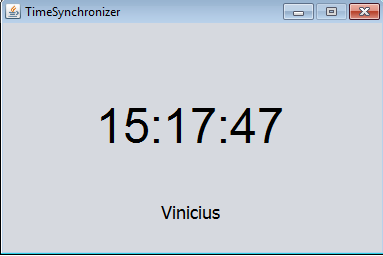
\includegraphics[scale = 0.45]{tela_inicial.eps}}
%	\qquad
%	\subfigure[home\_page][Home-Page com as opera��es dispon�veis.]{\includegraphics[scale = 0.45]{home_cliente.eps}}
%	\caption{Imagens do sistema desenvolvido.}
%	\label{sistemaimgs}
%	
%\end{figure}

\section{Introdu��o}

Na modernidade, tempo tornou-se um elemento precioso. N�o obstante, sua no��o � bastante difusa e, por diversas vezes, j� foi tema de discuss�es filos�ficas e alvo de pesquisas na F�sica. O que se sabe � que ele norteia a vida das sociedades e constitui-se como moeda de troca nas rela��es de trabalho.

Nos sistemas computacionais n�o � diferente. Ter uma refer�ncia para a execu��o das tarefas � importante. Essas tarefas podem ser as mais variadas: desde a cria��o de um arquivo at� a execu��o de uma tarefa previamente determinada, por exemplo. Entretanto, dispositivos diferentes podem mensurar instantes de maneira diferente e, com o passar do tempo, naturalmente atrasar ou adiantar. 

\section{Desenvolvimento}
\subsection{Sistemas Distribu�dos}
Coulouris define um sistema distribu�do no qual componentes de hardware ou software, localizados em computadores de uma rede, coordenam suas a��es e se comunicam por meio da troca de mensagens.

\subsection{Sincroniza��o em Sistemas Distribu�dos}

\subsection{}

\section{Resultados}

\section{Conclus�es}\label{concl}


\bibliographystyle{sbc}
\bibliography{sbc-template}

\end{document}
